\newpage
\begin{savequote}[108mm]
 ``Plan your work for today and every day, then work your plan.''
  \qauthor{Margaret Thatcher}
\end{savequote}
\chapter{Migration plan }
\label{chap:plans}
\vspace{-2cm}
%--------------------------------------------------------------------------------------
 
 Any successful migration must have a plan that approaches the process in phases that take the proper concerns into consideration at the proper time. This chapter  proposes a three phase process. The first phase is the planning process. The second phase is the actual migration. The third phase is implementation and testing. A majority of the work should be placed in the planning stage. An effort should be made to identify and devise solutions for any obstacles or challenges that should arise. The following outlines the phases of the migration process as shown in the Figure~\ref{fig:migrationplan}. 
 
\section{First Phase:Pre-migration}
 
 The pre-migration process is the most critical to the success of the project. In this phase, the goals and vision for the migration will form the guiding processes for the rest of the migration process. The needs of the organization must be the primary concern in the design and implementation of the new system. It is critical to have measurable goals and objectives. The organization must know where it is going before it can design a means to get there. The needs and goals of the business is the first, and perhaps most important phase of the process.                                                                                                                                

 \begin{figure}[H]
  \begin{center}
    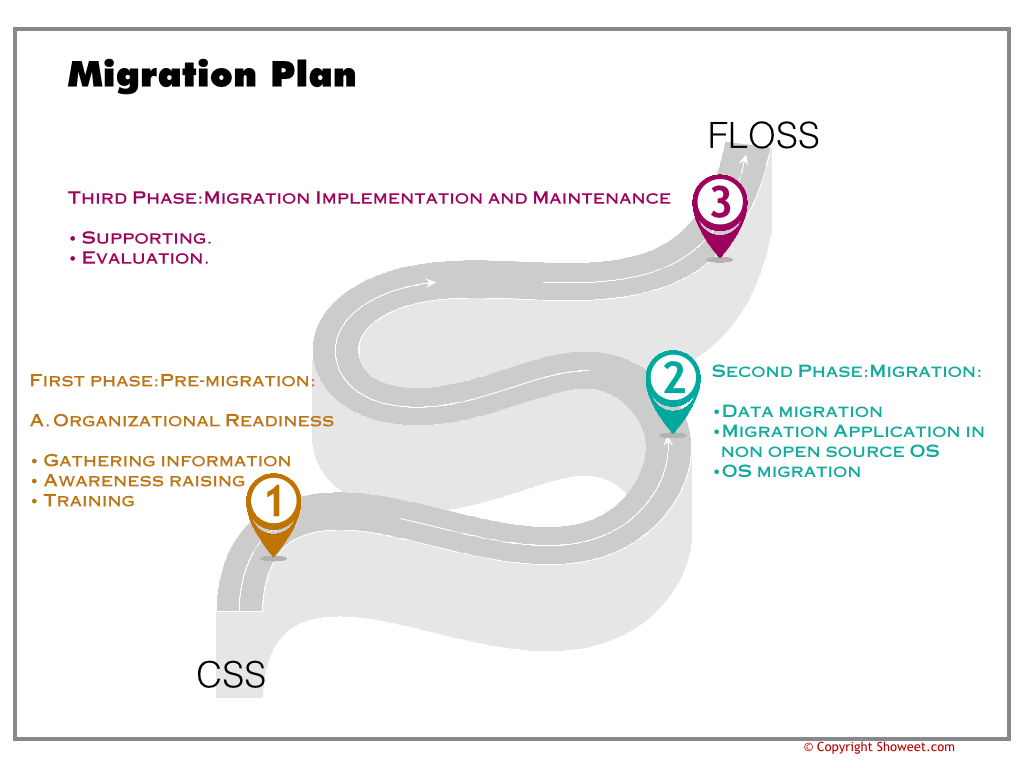
\includegraphics[scale=0.6,angle=90]{img/migrationplan.png}
      \caption{Migration plan}
      \label{fig:migrationplan}
  \end{center}
    \end{figure}
    
    \subsection{Organizational Readiness}
    
    Once the company has clear goals and knows what it needs the project to accomplish, it can then set about the task of assessing the readiness of the organization for the transition.
    
    \subsubsection{Gathering information}
    The first step in assessing organizational readiness is gathering information. 
    This must include a thorough audit to gather as much information as possible on existing hardware, software, and the needs that these component serve. The electrical and mechanical components of the building may have to be modified to accommodate the new system. All of these needs must be taken into consideration when assessing the readiness of the organization during the information gathering stage.
    
    Another component of readiness is personnel. An assessment needs to be made or current staff and any future staffing needs that will result from the migration to FLOSS. The organization needs to ask the question of whether they will need to hire any additional technical support, consultants, or training personnel in conjunction with the change. They need to assess whether these needs will be temporary or permanent changes to the organization. The organization also needs to determine if the current staff is prepared for the change and what needs to be done to get them ready. 
    
    There are many sources of information that should be considered. It is important to gather and compare as much information as possible from as many sources as possible. Personal interviews with various department executives to determine their needs is one source of information. The people that will be working directly with the new system will be the best sources of information within the organization.  In addition to sources of information within the organization, outside sources of information may be valuable as well. One can also examine case studies of similar migration projects. For instance, one might talk to others who have undergone similar changes in their organization. They can provide valuable insight as to any unforeseen challenges that one may face. One needs to gather information on the type of data that the organization utilizes and how it is organized within the current business system.  This information can be found by consulting with employees who produce the data and their managers.
    
    \subsubsection{Awareness raising and building a FLOSS community}
    
    \textit{ "Many people focus on encouraging more users to switch to free software. That's a useful thing to do. But that alone is not enough to bring us to freedoms that endure. If we gave everybody in the World free software today, but we failed to teach them about the four freedoms, then five years from now, would they still have free software?"}\footnote{Richard Stallman  presentation \url{http://blogs.fsfe.org/ciaran/?p=57}}
    
    Raising awareness in the organization goes beyond simple knowledge that the change will take place. Raising awareness includes getting people excited about the change and raising the level of support within the organization. It is about gaining managerial support and support on all levels of the organization. People must be made aware of the importance and advantages of the change for the organization. This support will be valuable if any challenges should arise during the process. 
    
    In addition to raising awareness within the organization, there also needs to be some consideration of community awareness too. Before involvement on the migration the community must have a clear understanding of the reasons to migrate.
    Building a FLOSS community, and participatory contributing are essential and recurring activities that enable FLOSS projects to persist. 

    The community will interact with the system, either directly or through organizational representatives. When public funds will be used, the public needs to be informed of the reasoning for the change and what they will mean for the community. Community awareness can be raised through public workshops, formal classes in schools, and town meetings. The mass media can also be used to raise public awareness through newspaper articles and stories by local television stories on the benefits of the new FLOSS. 
    
    \subsubsection{Training}
    The final consideration of the first phase concerns training. Prior to beginning implementation of the software, people must be trained on how to use it. In some cases, a majority of the changes will be on the back end of the system. The average user will not notice significant differences. In other cases, the migration will mean learning an entirely new of doing business. Without sufficient training, employees will be likely to have problems. This will lead to a dislike and lack of support for the new system. Proper training can help to eliminate these issues. 
    
    Training will include classroom training at the facility normally used by the organization for those purposes. and also can be by creating an e-learning environment. Training will include a variety of materials that cover the reason for the change, how the change will benefit the company, and how to operate the new system. It will give them hands on experience and will allow them time to ask any questions that they may have. Most importantly, it will provide them with information on where they can get help once the system is up and running.
    
    \section{Second Phase: Migration}
    
    The second phase of the migration process is moving the data and records from the old closed software to the new open platform. If compatibility issues exist, this is where many problems will occur.  A step by step and start with non critical systems; process needs to be devised that allows for as little disruption of the daily business routines of the organization as possible. This process will be different for every organization and for every migration. A plan for backing up date prior to migration is essential in case unforeseen circumstances should arise. The phases of the migration will cover four different areas. 
    
    \subsection{Data migration}
    
    Data migration to the new system is the most critical phase of the migration process. A data back-up plan is essential to prevent data loss. The ease or success of this phase of the plan depends on the compatibility and similarity of the two systems. If a large amount of data is involved, it may be possible to try a small-scale trial migration before attempting the large scale migration process. 
  
    It is important to divide the data into categories:
    \begin{enumerate}
    \item Data which can be get rid of.
     \item Data which must be kept it is useful and in open format such as PDF or Postscript, or can be easily translated into open format.
      \item  Data which must be kept but which is in a closed format which cannot be easily translated into an open one. This data may need copies of the CSS. The cost of these applications will need to be estimate.
    \end{enumerate}

    Data migration will entail moving the most critical data first. The application migration will take place in stages. First the lightweight, smaller applications will be migrated. Only the data that accompanies these small applications will be transferred first. Next, application and operating systems will be transferred. The data necessary at each of these junctures will be transferred at an appropriate time. The data migration process will be dependent on the timing and scheduling of the migration of the applications. 
    
    
    \subsection {Migration Application in non FLOSS OS}
    
    It is possible to run FLOSS and proprietary software in conjunction with each other, creating a highly customizable option that can fit almost any business need.
    
    The key to the success of this strategy is in the FLOSS. It is often prohibited to modify the proprietary software, but the FLOSS allows the developer to work around this obstacle without modifying the proprietary software. 
    
    The case study of the migration from closed to FLOSS in Zaragoza, Spain,   mention in detail later\footnote{Go to Section~\ref{Zaragoza}} provides a plan for migrating applications with as little interruption of business operations as possible. Following this example as a lead, applications must be prioritizes and moved according to their size.  The first applications to be migrated were lightweight  applications such as replacement of the Internet browser to one that is compatible with FLOSS. Next they replaced Outlook with Mozilla Thunderbird. They replaced their FTP client to one that was compatible with FLOSS. They also replaced Windows Media Player with VLC, a program that is more compatible with FLOSS. 
    
     Making these small changes first allowed people to be able to get used to the new system in a way that broke them in slowly. After the lighter weigh programs had been moved to FLOSS, they then moved the main office applications. During this phase, they would be using the new FLOSS system of all of their work. Moving the office applications is the phase that will have the greatest impact on the experiences of the employee. However, because they are familiar with the new system from the migration of lightweight applications, it is expected to make transition of the office system easier. This staged approach will yield and easier transition for the employees who will use the new FLOSS system.          
  
   \subsection{OS migration}
    \label{opensource_OS} 
    The operating system was the last item to be moved.  There are many details that cannot be provided without information on the two operating systems involved. Operating system migration is a specialized field and there are many nuances to the process. It is recommended that a consultant be used for this part of the migration process. There are many choices for operating systems that can support FLOSS.
    
    Linux is the most common operating system for both FLOSS and hybrid systems. Linux is highly configurable, making it the system of choice for many large scale operations. However, this is not the only operating system choice. The most important consideration when choosing a new operating system for a backbone is to consider the current and future needs of the organization. A system that can be easily expanded in the future is the most economical choice. Consultants and outside contractors are the most valuable resource in the operating system migration. 
    
     \section{Third Phase: Migration Implementation and Maintenance}
     \label{Implementation}
     
     The third phase of the migration is final implementation. If you have taken the time and given the proper attention to these previous phases, they may be a time for celebrating the new system. Prior to full implementation, the new system should be tested any bugs addressed. The first few days of weeks may be difficult as everyone learns the new system. Supporting will play a role in getting through this initial phase. 
     \subsection {Supporting}
     
     It is essential to consider having enough support available during all of this phase. These supports can be internal or external to the organization. It may be possible to transition these support personnel to permanent technical support. 
     
     After the migration is complete, a support system will be set up for employees who use the system on a daily basis. This will include a special help line number that they can call to have their questions answered. Telephone support is expected to be one of the main form of support used in a majority of the situations. 	There will also be a support website set up that will have a troubleshooting tool that can walk customers through some of the most common problems that they will encounter. They will also have the option of contacting the support department through email or chat. Employees will have many different avenues to contact support, depending on the urgency of their issue. 
     
     Once this initial learning phase is complete, the organization can then turn its attention to maintenance of the new system and any improvements that it wishes to make in the future. The maintenance that needs to be performed depends on the system that is chosen as the FLOSS platform, the amount of data processed, and other factors. This will be an ongoing process throughout the lifespan of the system. The maintenance plan will be set into a formal written form that outlines all of the procedures and the schedule in which they will be performed. 

